\documentclass[../main.tex]{subfiles}
\begin{document}
\chapter{Iteration and Recursion}
\label{chapter_iteration_recursion}
\begin{chapquote}
{Niklaus Wirth, \textit{Algorithms + Data Structures = Programs, 1976}}
``The power of recursion evidently lies in the possibility of defining an infinite set of objects by a finite statement. In the same manner, an infinite number of computations can be described by a finite recursive program, even if this program contains no explicit repetitions.''
\end{chapquote}

\section{Introduction}
\label{iteration_recursion_introduction}
\begin{figure}[h]
    \centering
    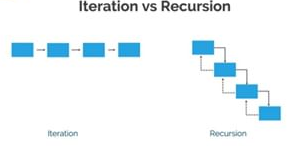
\includegraphics[width = 0.7\columnwidth]{fig/iteration_recursion.png}
    \caption{Iteration vs recursion: in recursion, the line denotes the top-down process and the dashed line is the bottom-up process. }
    \label{fig:iteration_vs_recursion}
\end{figure}
In computer science, software programs can be categorized as either \textit{iteration} or \textit{recursion}, thus making iteration and recursion as the topmost level of concepts in software development and the very first base for us to study computer science techniques. Iteration refers to a \textit{looping} process which repeats some part of the code until a certain condition is met. Recursion, similarly, needs to stop at a certain condition, but it replaces the loop with recursive function calls; meaning  a function calls itself from within its own code. The process is shown in Fig.~\ref{fig:iteration_vs_recursion}. 

Do you still have the feeling that you seemingly already understand the iteration even without code, but what is recursion exactly? Recursion can be a bit of challenging for beginners, it differs from our normal way of thinking. It is a bit of similar to the vision of being in the restroom which has two mirrors abrest on each side and facing each other, we see multiple images of the things in front of each mirror, and these images usually appear from large to small. This is similar to recursion. The relation between these recurred images can be called \textit{recurrence relation}. 

Understanding recursion and learning basic rules to solve recurrence relation are two of the most purposes in this chapter. Thus, we organize the content of this chapter following this trend:
\begin{enumerate}
    \item Section.~\ref{sec_iteration_recursion} will first address our question by analyzing the recursion mechanism within the computer program, and we further understand the different between by seeing example of factorial series and examines the pros and cons of each. 
    \item Section.~\ref{sec_recursion} advances our knowledge about recursion by studying the recurrence relation, including its definition, categorization and addressing how to solve recurrence relation. 
    \item Section.~\ref{sec_iter_recur_examples} gives us two examples to see how iteration and recursion works in real practice. 
\end{enumerate} 
\begin{importantnote}
Deduce(find) the recurrence relation and sometimes solves it is a key step in algorithm design and problem solving,  solving the recurrence time relation is important to  algorithm analysis. 
\end{importantnote}
%we will first andwer the question: recursion handles function calls in two passes -- \textit{top-down} and \textit{bottom-up}. In the top-down process, recursion starts from the entrance of the program, call itself   it is composed of two passes:Thus, in this chapter, we   The purpose of this chapter is to understand how iteration and recursion works in algorithms and software developing. Especially, to understand how recursion works, and we also include the most common usage of being recursion. 

% \section{Iteration and Recursion}
% \label{sec_iteration_recursion}
In this section, we first learn iteration and Python Syntax that can be used to implement. We then examine a classic and elementary example--Factorial sequence to catch a glimpse of how iteration and recursion can be applied to solve this problem. Then, we discuss more details about recursion. We end this section by comparing iteration and recursion; their pros and cons and their relation between. 

\section{Iteration}
In simple terms, an iterative function is one that loops to repeat some part of the code. In Python, the loops can be expressed with \texttt{for} and \texttt{while} loop. 

Enumerating the number from $1$ to $10$ is a simple iteration. Implementation wise:
\begin{itemize}
    \item \texttt{for} usually is used together with function \texttt{range(start, stop, step)} which creates a sequence of numbers from \texttt{start} to \texttt{stop} in range $[start, end)$, and increments by $step$ (1 by default). Thus, we need to set \texttt{start} as 1, and \texttt{end} as 11 to get numbers from 1 to 10. 
\begin{lstlisting}[language=Python]
# enumerate 1 to 10 with for loop
for i in range(1, 11):
  print(i, end=' ')
\end{lstlisting}
\item \texttt{while} is used with syntax
\begin{lstlisting}[numbers=none]
while expression
    statement
\end{lstlisting}
In our case, we need to set start condition which is $i=1$, and the expression will be limiting $i <= 10$. In the statement, we need to manually increment the variable \texttt{i} so that we wont not end up with infinite loop.
\begin{lstlisting}[language=Python]
i = 1
while i <= 10:
  print(i, end = ' ')
  i += 1
\end{lstlisting}
\end{itemize}

\section{Factorial Sequence}  The factorial of a positive integer $n$, denoted by $n!$, is the product of all positive integers less than or equal to $n$:
\begin{lstlisting}[numbers=none]
For example: 
5! = 5 \times 4 \times 3 \times 2 \times 1 = 120.
0! = 1
\end{lstlisting}
% In this section, we are going to approach the problem using both iteration and recursion, conceptually and implementally. 
To compute the factorial sequence at $n$, we need to know the factorial sequence at $n-1$, which can be expressed as a \textit{recurrence relation}, that $n!= n \times (n-1)!$). 
\begin{itemize}
    \item Solving with iteration: we use a \texttt{for} loop starts at 1 up till $n$ so that we eventually build up our answer at $n$. We use a variable \texttt{ans} to save the factorial result for each number, and once the program stops, \texttt{ans} gives the result of our factorial for $n$.
\begin{lstlisting}[language=Python]
def factorial_iterative(n):
  ans = 1
  for i in range(1, n+1):
    ans = ans * i
  return ans
\end{lstlisting}
\item Solving with recursion: we start to call a recursive function at $n$, within this function, we can itself but instead with $n-1$ just as shown in the recurrence relation. We then multiply this recursive call with $n$. We need to define a bottom, which is the end condition for the recursive function calls to avoid infinite loop. In this case, it bottoms out at $n=1$, which we can know its answer would be $1$, thus we return 1 to stop further function calls and recursively return to its upmost level.
\begin{lstlisting}[language=Python]
def factorial_recursive(n):
  if n == 1:
    return 1
  return n * factorial_recursive(n-1)
\end{lstlisting}
\end{itemize}

\section{Recursion}
In this section, we reveal how the recursion mechanism works: function calls and stack, two passes. 
\label{sec_recursion}
\begin{figure}[!ht]
    \centering
    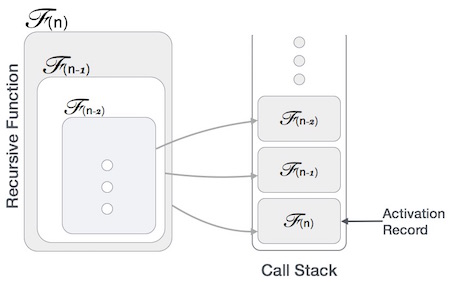
\includegraphics[width=0.6\columnwidth]{fig/activation_records.png}
    \caption{Call stack of recursion function}
    \label{fig:call_stack_recursion_function}
\end{figure}
\paragraph{Two Elements}
When a routine calls itself either directly or indirectly, it is said to be making a recursive function call. The basic idea behind solving problems via recursion is to break the instance of the problem into smaller and smaller instances until the instances are so small they can be solved trivially. We can view a recursive routine as consisting of two parts. 
\begin{itemize}
    \item Recursive Calls: As in the factorial sequence, when the instance of the problem is still too large to solve directly, we recursive call this function itself to solve problems of smaller size. Then the result returned from the recursive calls are used to build upon the result of the upper level using \textit{recurrence relation}. For example, If we use $f(n)$ to denote the factorial at $n$, the recurrence relation would be $f(n)=n\times f(n-1), n>0$.
    \item End/Basis  Cases: The above resursive call needs to bottom-out; stop when the instance is so small to be solved directly. This stop condition is called end/basic case. Without this case, the recursion will continue to dive infinitely deep and eventually we run of memory and get a crash. A recursive function can have one or more base cases. In the example of factorial, the base case is when $n=0$, by definition $0!=1$.
\end{itemize}


\paragraph{Recursive Calls and Stacks}
The recursive function calls of the recursive factorial we implemented in the last section can be demonstrated as Fig.~\ref{fig:call_stack_recursion_function}. 

The execution of recursive function $f(n)$ will pay two visits to each resursive function $f(i), i \in [1, n]$ through two passes: \textit{top-down} and \textit{bottom-up} as we have illustrated in Fig.~\ref{fig:iteration_vs_recursion}. The recursive function handles this process via a \textit{stack} data structure which follows a Last In First Out (LIFO) principle to record all function calls.

\begin{itemize}
    \item In the top-down pass, each recursive function's execution context is ``pushed'' into the stack in the order of $f(n)$, $f(n-1)$, ..., $f(1)$. The process ends till it hits to the end case $f(0)$, which will not be ``pushed'' into the stack but execution some code and \texttt{returns} value(s). The end case marks as the start of the bottom-up process.

\item In the bottom-up pass, the recursive function's execution context in the stack is ``poped'' off the stack in a reversed order: $f(1)$, ..., $f(n-1)$, $f(n)$. And $f(1)$ takes the returned value from the base case to construct its value using the recurrence relation. Then it returns its value up to the next recursive function $f(2)$. This whole process ends at $f(n)$ which returns its value. 
\end{itemize}

\paragraph{How Import Recursion Is?} 
Recursion is a very powerful and fundamental technique, and it is basis for several other design principles, such as:
\begin{itemize}
    \item Divide and Conquer (Chapter.~\ref{chapter_divide_conquer}).
    \item Recursive Search, such as Tree Traversal and graph search.
    \item Dynamic Programming (Chapter.~\ref{chapter_dynamic-programming}.
    \item Combinatorics such as enumeration (permutation and combination) and branch and bound etc.
    \item Some classes of greedy algorithms.
\end{itemize}
It also supports the proof of correctness of algorithms via mathematical induction, and consistently arise in the algorithm complexity analysis. We shall see through out this book and will end up drawing this conclusion ourselves. 

\paragraph{Practical Guideline}
In real algorithmic problem solving, different process normally has different usage. 
   
In top-down process we do:
\begin{enumerate}
    \item Break problems into smaller problems, there are different ways of ``breaking'' and depends on which, they can either be \textit{divide and conquer} or \textit{decrease and conquer} which we will further expand in Chapter.~\ref{} and \ref{}. Divide and conquer will divide the problems into disjoint subproblems, whereas in decrease and conquer, the problems 
    \item Searching: visit nodes in non-linear data structures (graph/tree), visit nodes in linear data structures. Also, at the same time, we can use \textbf{pass by reference} to track the state change such as the traveled path in the path related graph algorithms. 
\end{enumerate}


In bottom-up process, we can either return \texttt{None} or \texttt{variables}. Assume if we already used \textbf{pass by reference} to tack the change of state, then it is not necessarily to return variables. In some scenario, tracking states with by passing by reference can be more easier and more intuitive. For example, in the graph algorithm, we mostly like to use this method. 

\paragraph{Tail Recursion}
This is also called \textit{tail recursion}  where the function calls itself at the end (``tail'') of the function in which no computation is done after the return of recursive call. Many compilers optimize to change a recursive call to a tail recursive or an iterative call.

%Returning variables 
% \begin{enumerate}
%     \item Using rreturn None: Simply return to the upper level if we already used \textbf{pass by reference} to tack the change of state. 
%     \item return variables: We get the result of the next recursive function call and using the recurrence relation to construct the result of current function. if we have return result, we do process of these results with current state and return to the upper level. In divide and conquer, we mostly likely need to merge its results. For iteration, this process gives the iteration process the backward traveling process. 
% \end{enumerate}

% \paragraph{Examples of Applications}
% For iteration, the top-down process is visiting nodes in 'forwarding' direction, and the bottom-up process on the other hand functions as a reverse visiting process. This makes a linear data structures function as a doubly linked list, and make a one direction tree structure function as one with parent. Here we list some examples that used recursive so that we can go backward:
% \begin{enumerate}
%     \item 2. Add Two Numbers
% \end{enumerate}

\section{Iteration VS Recursion}

\paragraph{Stack Overflow Problem} 
In our example, if we call function \texttt{factorial\_recursive()} with $n=1000$, Python would have complain an error as:
\begin{lstlisting}
RecursionError: maximum recursion depth exceeded in comparison
\end{lstlisting}
which is a \textit{stack overflow} problem.
A stack overflow is when we run out of memory to hold items in the stack. These situations can incur the stack overflow problem:
\begin{enumerate}
    \item No base case is defined. 
    \item The recursion is too deep which is out of the assigned memory limit of the executing machine. 
\end{enumerate}
\paragraph{Stack Overflow for Recursive Function and Iterative Implementation} According to Wikipedia, in software, a stack overflow occurs if the call stack pointer exceeds the stack bound. The call stack may consist of a limited amount of address space, often determined at the start of the program depending on many factors, including the programming language, machine architecture, multi-threading, and amount of available memory. When a program attemps to use more space than is available on the call stack, the stack is said to \textit{overflow}, typically resulting in a program crash. The very deep recursive function is faced with the threat of stack overflow. And the only way we can fix it is by transforming the recursion into a loop and storing the function arguments in an explicit stack data structure, this is often called the iterative implementation which corresponds to the recursive implementation. 

We need to follow these points:
\begin{enumerate}
    \item End condition, Base Cases and Return Values: either return an answer for base cases or None, and used to end the recursive calls.  
    \item Parameters: parameters include: data needed to implement the function, current paths, the global answers and so on. 
    \item Variables: What the \textbf{local} and {global} variables. In Python any pointer type of data can be used as global variable global result putting in the parameters. 
    \item Construct current result: when to collect the results from subtree and combine to get the result for current node.
    \item Check the depth: if the program will lead to the heap stack overflow.
\end{enumerate}


\paragraph{Conversion} For a given problem, conversion between iteration and recursion is possible, but the difficulty of the conversion is highly dependable on specific problem context. For example, the iteration of a range of numbers can be represented with recurrence relation $T(n)=T(n-1)+1$. On the side of implementation, some recursion and iteration can be easily converted between such as linear search; in some other cases, it takes more tricks and requires more sophisticated data structures to assist the conversion, such as in the iterative implementation of the recursive depth-first-search, it uses stack. Do not worry about these concepts here, as you flip more pages in the book, you will know and start to think better. 

\paragraph{Tail recursion and Optimization}

In a typical recursive function, we usually make the recursive calls first, and then take the return value of the recursive call to calculate the result. Therefore, we only get the final result after all the recursive calls have returned some value. But in a tail recursive function, the various calculations and statements are performed first and the recursive call to the function is made after that. By doing this, we pass the results of the current step to the next recursive call to the function. Hence, the last statement in a Tail recursive function is the recursive call to the function.
This means that when we perform the next recursive call to the function, the current stack frame (occupied by the current function call) is not needed anymore. This allows us to optimize the code. We Simply reuse the current stack frame for the next recursive step and repeat this process for all the other function calls.

Using regular recursion, each recursive call pushes another entry onto the call stack. When the functions return, they are popped from the stack. In the case of tail recursion, we can optimize it so that only one stack entry is used for all the recursive calls of the function. This means that even on large inputs, there can be no stack overflow. This is called Tail recursion optimization.

Languages such as lisp and c/c++ have this sort of optimization. But, the Python interpreter doesn’t perform tail recursion optimization. Due to this, the recursion limit of python is usually set to a small value (approx, $10^4$). This means that when you provide a large input to the recursive function, you will get an error. This is done to avoid a stack overflow. The Python interpreter limits the recursion limit so that infinite recursions are avoided.

 
\paragraph{Handling recursion limit}
The ``sys module'' in Python provides a function called \texttt{setrecursionlimit()} to modify the recursion limit in Python. It takes one parameter, the value of the new recursion limit. By default, this value is usually $10^4$. If you are dealing with large inputs, you can set it to, $10^6$ so that large inputs can be handled without any errors.


% \section{Hands-on Examples}
% \label{sec_iter_recur_examples}

\section{Exercises}
\begin{enumerate}
    \item Compute factorial sequence using \texttt{while} loop.
\end{enumerate}

\section{Summary}
If a cursive algorithm can be further optimized, the optimization method can either be divide and conquer or decrease and conquer. We have put much effort into solving recurrence relation of both: the linear recurrence relation for decrease and conquer, the divide and conquer recurrence relation for divide and conquer.  Right now, do not struggle and eager to know what is divide or decrease and conquer, it will be explained in the next two chapters. 
    % A conditional statement decides the termination of recursion while a control variable’s value decide the termination of the iteration statement (except in the case of a while loop).
    % Infinite recursion can lead to system crash whereas, infinite iteration consumes CPU cycles.
    % Recursion repeatedly invokes the mechanism, and consequently the overhead, of method calls. This can be expensive in both processor time and memory space while iteration doesn’t.
    % Recursion makes code smaller while iteration makes it longer.
\end{document}